\chapter{Introduction}
\label{chap:introduction}

\textit{
This chapter is going to introduce the context of the project, including a brief overview of all the different parts that will be discussed in the project. It will also break down a series of objectives to be carried out during the realization of the project. Moreover, it will introduce the structure of the document with an overview of each chapter.}



\clearpage

\section{Context and motivation}
\label{sec:context}

 %-------------------Pandemia de Covid --> efectos secundarios en la salud mental --> problema importante a ser tratado -------------------
% Articulos para esta parte
% 1- https://www.scielosp.org/article/rpmesp/2020.v37n2/327-334/es/
% Conector - https://www.proquest.com/docview/2605236970/fulltextPDF/3291A3310F4C45D6PQ/1?accountid=14712


On 14 March 2020, due to the global pandemic caused by COVID-19, Spain entered a period of quarantine for several months, during which people had to stay indoors, with reduced social interaction, limited to people living in the same household. Confirmed cases and deaths caused by the virus increased rapidly and as a result of these reasons, the population experienced the development of psychological problems such as anxiety, depression and stress, as studies have shown~\cite{ramirez2021repercusiones}.

The effects of the measures put in place to combat this pandemic have had a notable impact on mental health, increasing the development of inherent illnesses and psychological problems, such as Eating Disorders. The risk of suffering from one of these disorders has increased, with patients with no preexisting symptoms being able to develop one of these disorders under certain circumstances, as emotional eating is related to biological, psychological and social factors, and the COVID-19 pandemic has been the perfect breeding ground for these types of problems to develop or grow worse~\cite{dos2022emotional}.

Different studies have shed light on this situation and its importance, as people are having problems with the management of their emotions, which has an impact on their well-being and in particular on what they eat, so it is very important to raise awareness and implement measures to combat the side effects that this pandemic will have in the long term, as the longer it takes, the worse these problems will become~\cite{touyz2020eating}.


%-------------------Definition -------------------

For setting the ground of the main topic tackled in this Master Thesis, the definition of disorders called Eating Disorders is the following:  

\textit{Eating Disorders are a group of mental disorders that are driven by the development of behaviors aimed at weight control and an altered eating behaviour. This alteration causes physical and psycho-social functioning problems. EDs are illnesses whose main traits are distorted eating behavior and extreme concern with self-image and body weight. The main representation of these disorders are Anorexia Nervosa (AN), Bulimia Nervosa (BN) and ED not otherwise specified, which includes binge eating disorder}~\cite{baldares2013trastornos}.


 %-------------------Los TCAs estan en alza por x o Y despues de la pandemia, siendo un problema sobre todo en las mujeres jovenes -------------------
% 2- https://onlinelibrary.wiley.com/doi/full/10.1002/eat.23704?casa_token=yKMsm3-JKHYAAAAA%3A_3ZlIvnwecCYorG7JkCITwg2c5b6igm_cyBSPWj7qEvycaCiYDfq0wx3FHOZ1XVi91N3Gi-VCx9JqXU
% Interesantisimo: https://www.behavioralpsycho.com/wp-content/uploads/2021/09/08.Vall_29-2Es.pdf

% Se pueden usar para extender
% NO USADO https://dialnet.unirioja.es/servlet/articulo?codigo=8260225
% NO USADO evolucion EDs en COVID https://aepnya.eu/index.php/revistaaepnya/article/view/850
% NO USADO lo mismo https://www.aepnya.eu/index.php/revistaaepnya/article/view/402

These studies mentioned above are not based on conjecture, but rather, through an exhaustive and quantitative analysis, such as that carried out in various studies such as~\cite{j2022impact} or~\cite{vall2021impacto}, it has been shown that subjects suffering from an Eating Disorder have experienced deteriorating symptoms, increased isolation and, as a consequence, an increase in hospital admissions as a result of COVID-19. Specifically, it has been found that on average admissions have increased by 48\% compared to pre-pandemic times. In addition, it was found that 36\% of patients' symptoms increased, especially those related to anxiety and depression.

It has also been found that the pandemic has had a major impact on young women between 14 and 35 years of age, as shown in demographic studies carried out~\cite{vall2021impacto} which report severe or very severe levels of illness and symptoms, namely 30.8\% of the sample analysed suffered from depression, 25.4\% suffered from anxiety and 20.5\% from stress. Significant gender differences were found in terms of eating disorders, and it was found that life events that generate stress are related to eating disorders.

In the aforementioned study, the data were processed and a model was generated that related the different terms studied in this Master Thesis, as can be seen in Figure \ref{fig:vall_diagram}. It is possible to appreciate the correlation between them that was observed in the study carried out, being negative between psychological wellbeing and the symptomatologies that occur in mental illnesses. Furthermore, psychological wellbeing is also related to different factors such as self-esteem, concern for appearance and self-care, the first two being the ones that have the greatest weight on wellbeing.
%% AÑADIR ALGO MAS DE LA FIGURA??

\begin{figure}[!htp]
    \centering
    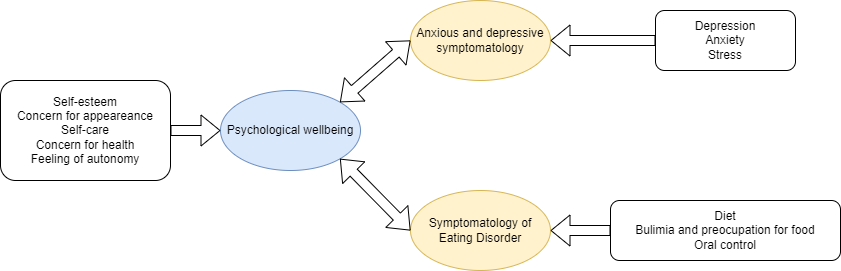
\includegraphics[scale=0.5]{img/introduction/vall_diagram.png}
    %\begin{minipage}{1}
    %\footnotesize
    %\emph{YOUR NOTES}
    %\end{minipage}
    \caption{Structural equation model relating the psychological impact of confinement to anxiety, depression and eating disorder symptoms~\cite{vall2021impacto}.}
    \label{fig:vall_diagram}
\end{figure}
% traducit y meter diagrama de Vall_29 Figura 1



% ######################## NO SE HA METIDO ########################################
% -------------------Problemas que constan los TCAs --> nivel sanitario y sociologico -------------------
%EAT-26, EAT-40 y SCOFF --> instrumentos para medir frecuencias, chequear para dar numeros en este apartado
% ##################################################################################


% -------------------Social networks and eating disorders (check resources de anteproyecto) -------------------
%Articulo covid + tecnologia + enfermedades mentales: http://www.dspace.uce.edu.ec/handle/25000/25604
% NO USADO -  carta a director anorexia: https://www.scielo.cl/scielo.php?pid=S2452-60532022005000319&script=sci_arttext


\myparagraph{Motivation}
This Master Thesis have been developed on the topic of Mental Health and the relationship of this with technology, social networks and information related to COVID-19 with the aim of knowing the impact of this in which, after an exhaustive literature review, it has been determined that there is a significant association between inappropriate and prolonged use of social networks and the effects of mental health, finding mainly anxious, depressive, stressful and compulsive patterns among others. Therefore, they have determined that social networks can lead to public health problems~\cite{pozo2022impacto}.

From the above, the importance of Eating Disorders after the pandemic has been understood, especially in young women today. Technology and in particular social networks, as a means of communication and expression, play a decisive role in the well-being of current society and particularly, as studied, in the development of these disorders.

Thanks to these, large amounts of information can be extracted and subsequently analysed, processed and used to improve the most critical part of these Eating Disorders, detection. The proposed tool will be used to help people to detect and analyse profiles of users potentially suffering from a disorder, in order to speed up the clinical diagnosis process, which is a key factor to take into account when treating a patient with this type of problem.

%\clearpage

\section{Project goals}
\label{sec:goals}
The goals of this Master Thesis have been designed from the beginning towards developing a social contribution that tackles one problem from the current society: Eating Disorders. With that in mind, the main goal of the present project is to \textbf{develop of a system for the analysis and detection of Eating Disorder-related mental health problems in social networks}. The application will integrate artificial intelligence technologies such as Natural Language Processing (NLP) and machine learning to detect these problems working with user data extracted from social media. The purpose of this tool is the \textbf{detection and analysis of user publications referring to Eating Behavior Disorders on social networks}. For this, several sub tasks are required:

\begin{itemize}
    \item Data collection, processing and analysis
    \item Design and implementation of machine learning models able to detect eating disorders from social media
    \item Training and evaluation the proposed models using the obtained datasets
    \item Development of a web application that integrates the proposed models for detecting and analyzing eating disorders
\end{itemize}

%\clearpage

\section{Structure of this document}

The remaining of this document is structured as follows:

\textbf{\textit{Chapter 2. State of art}}

\textbf{\textit{Chapter 3. Architecture}} 

\textbf{\textit{Chapter 4. Case study}}

\textbf{\textit{Chapter 5. Conclusions}} 